%\section{Recognition GT annotation}

%\subsection{Introduction Thingy}

The goal of this section is to obtain a groundtruth annotation for fish recognition. 
More specifically, we want to know which fish images belong to the same species, along with
the species names. 
This allows us to train and evaluate our fish recognition methods in the F4K project. 
In order to support the manual labelling of images, we propose to use an automatic clustering method to 
groups and retrieve similar images, which allows us to label large dataset in an efficient manner. 

This section is organised as follows: 
We start with a discussion of the fish clustering method that is used to support the labelling task.
%Firstly, we will discuss the fish clustering method that is used to support the labelling task. 
We then explain how we combine the clustering method with the annotation interfaces to support manual annotation work.
%Secondly, we explain how we combined the clustering method to the user interface to support the labelling task. 
Two types of annotation interfaces are defined: i)~the interface for normal annotators to label fish images; 
and ii)~the interface for marine biologists to verify the obtained labels.
%Thirdly, we will discussed the interface of the normal users to label our databases. Finally, we discussed
%the interface for biologist to verify the obtain labelling. 
\todo{We close this section with a discussion of the quality of the labels obtained.}


%\todo{Jiyin: I think we should have a section to evaluate the quality of the labels. The general idea is as follows.
%The biologists provide the labels of species as well as the cluster labels. Using these cluster labels we can 
%do two things: 1)evaluate the automatic clustering results (or finding the parameters); 2) evaluate the non-expert
%clustering cleaning/merging results.}    


%\subsection{First method to determine the similarity between fish}
\todo{I changed the subsection titles here, the original one was ``First method to determine the similarity between fish''. 
It's confusing: why is it a ``first'' method? as there doesn't seem to have a ``second'' method ....}

\subsection{Fish Clustering}

\subsubsection{Measuring similarity between fish images}
The fish clustering method starts with the assumption that the segmentation of the 
fish is correctly performed. In the case that we do not have groundtruth segmentation data, we can 
use visual inspection to manual remove failures in the segmentation from the dataset, this migt however 
be very time consuming.\todo{Do you mean manually remove the wrong segmentations? What's the relation
of this to the similarity measure?}

\todo{It is confusing here whether we are talking about similarity measures/fish representations or clustering method.I thought we
are talking about similarity measures/fish representations...}
In order to compare fish, we need a method which is also able to compare unseen fish species with
already know species in the dataset.
The similarity method needs to be invariant against a lot of variantions because of the 
uncontrolled nature of the video recording. The last requirement on the method is that it
must be able to deal with objects which are quite similar, as opposed to most methods in image 
retrieval where the classes with are quite dissimilar (car, building, people, etc). 
To compute the similarity between images, we use a method that is very similar to the method described in 
\cite{goldberger_unsupervised_2006}.


The feature used for fish recognition are the color of the fish, the texture of the fish and the fish contour.
In the case of color, we transform all the pixel values of the segmented fish to HSV (Hue, Saturtion, 
Value), for the Hue channel two values are used, namely the sine and cosine of the Hue channel. This removes the big 
difference between the different red values because of the cylindrical color definition. Using all the 4 dimensional
pixel values $X = \{x_{1},\dots,x_{N}\}$ in the segmented image, we fit a Gaussian Mixture Model (GMM) $f(x)$, using 
the Expectation Maximalization 
algorithm described in \cite{zivkovic_recursive_2004}, which uses Minimum Description Lenght to automatically determine 
the number of Guassian density functions. For the texture, a GMM is fitted to the magnitude and the orientation of the 
Canny filter at each pixel in the segmented fish. We also fitted a GMM on the curvature
scale space representation of the fish contour, where we use the points on lines given by the curvature 
scale space of the fish contour as input vector to fit a GMM. The advantage of using the curvature scale space is that
it gives an invariant representation for most affine image transformations on the contour. We use 
Gaussian Mixture Model (GMM) because they give us an invariant representation which is able to make a model
of the presented data, allowing the method to discover new species without needing models of these species
by forehand. 
In \cite{goldberger_unsupervised_2006}, the similarity between two GMMs $(f_{1},f_{2})$ is determined by using a Monte-Carol
simulation to approximate the Kullback-Liebler divergence:

\begin{equation}
 D(f_{1} \Vert f_{2}) = \int f_{1} \log \frac{f_{1}}{f_{2}} \approx \frac{1}{N} \sum_{t=1}^{N} \log \frac{f_{1}(x_t)}{f_{2}(x_t)} 
\end{equation}
\begin{equation} 
 S(f_{1},f_{2}) = D(f_{1} \Vert f_{2}) + D(f_{2} \Vert f_{1})
\end{equation}

We use the symmetric version of the KL-divergence (Equation 2) to measure the similarity between different 
fish images. Given the three different kind of features (colour,texture and contour), we obtain three different 
KL-divergences which we sum together to get the final similarity measure. 

\subsubsection{\textbf{Clustering based on similarity between objects}}

In order to compute clusters based on the similarity between objects, we use Affinity Propagation \cite{frey_clustering_2007}. 
Although in \cite{goldberger_unsupervised_2006}, a method for clustering is described to combine the GMMs, 
the Affinity Propagation method in \cite{frey_clustering_2007} scales better on large databases.
The Affinity Propagation is a graph based clustering method. %which can automatically find 
%clusters given a matrix of similarity measurements. 
This clustering method passes
messages around to determine the responsibility and availability. The message of responsibility between point
$i$ and $k$ reflects how well suited point $k$ represents point $i$. The availability message between point
$i$ and $k$ indicates how appropriate it is for point $i$ to choose point $k$ as representative. The final 
outcomes of the clustering method are clusters of fish images which have one image as a representative 
image.

The representative image is important in our interface for normal annotators because we use this image to link 
the clusters together.\todo{What does ``link the clusters together'' mean?} See below.
However, although \cite{frey_clustering_2007} gives us representative image
for each cluster, this does not mean that other clustering methods can not be used. For instance by using K-means
clustering, it is easy to select the images closest to the mean of the cluster as representative; 
in addition, using a random images in the cluster as representative should also work. 

\begin{figure}
\begin{center}
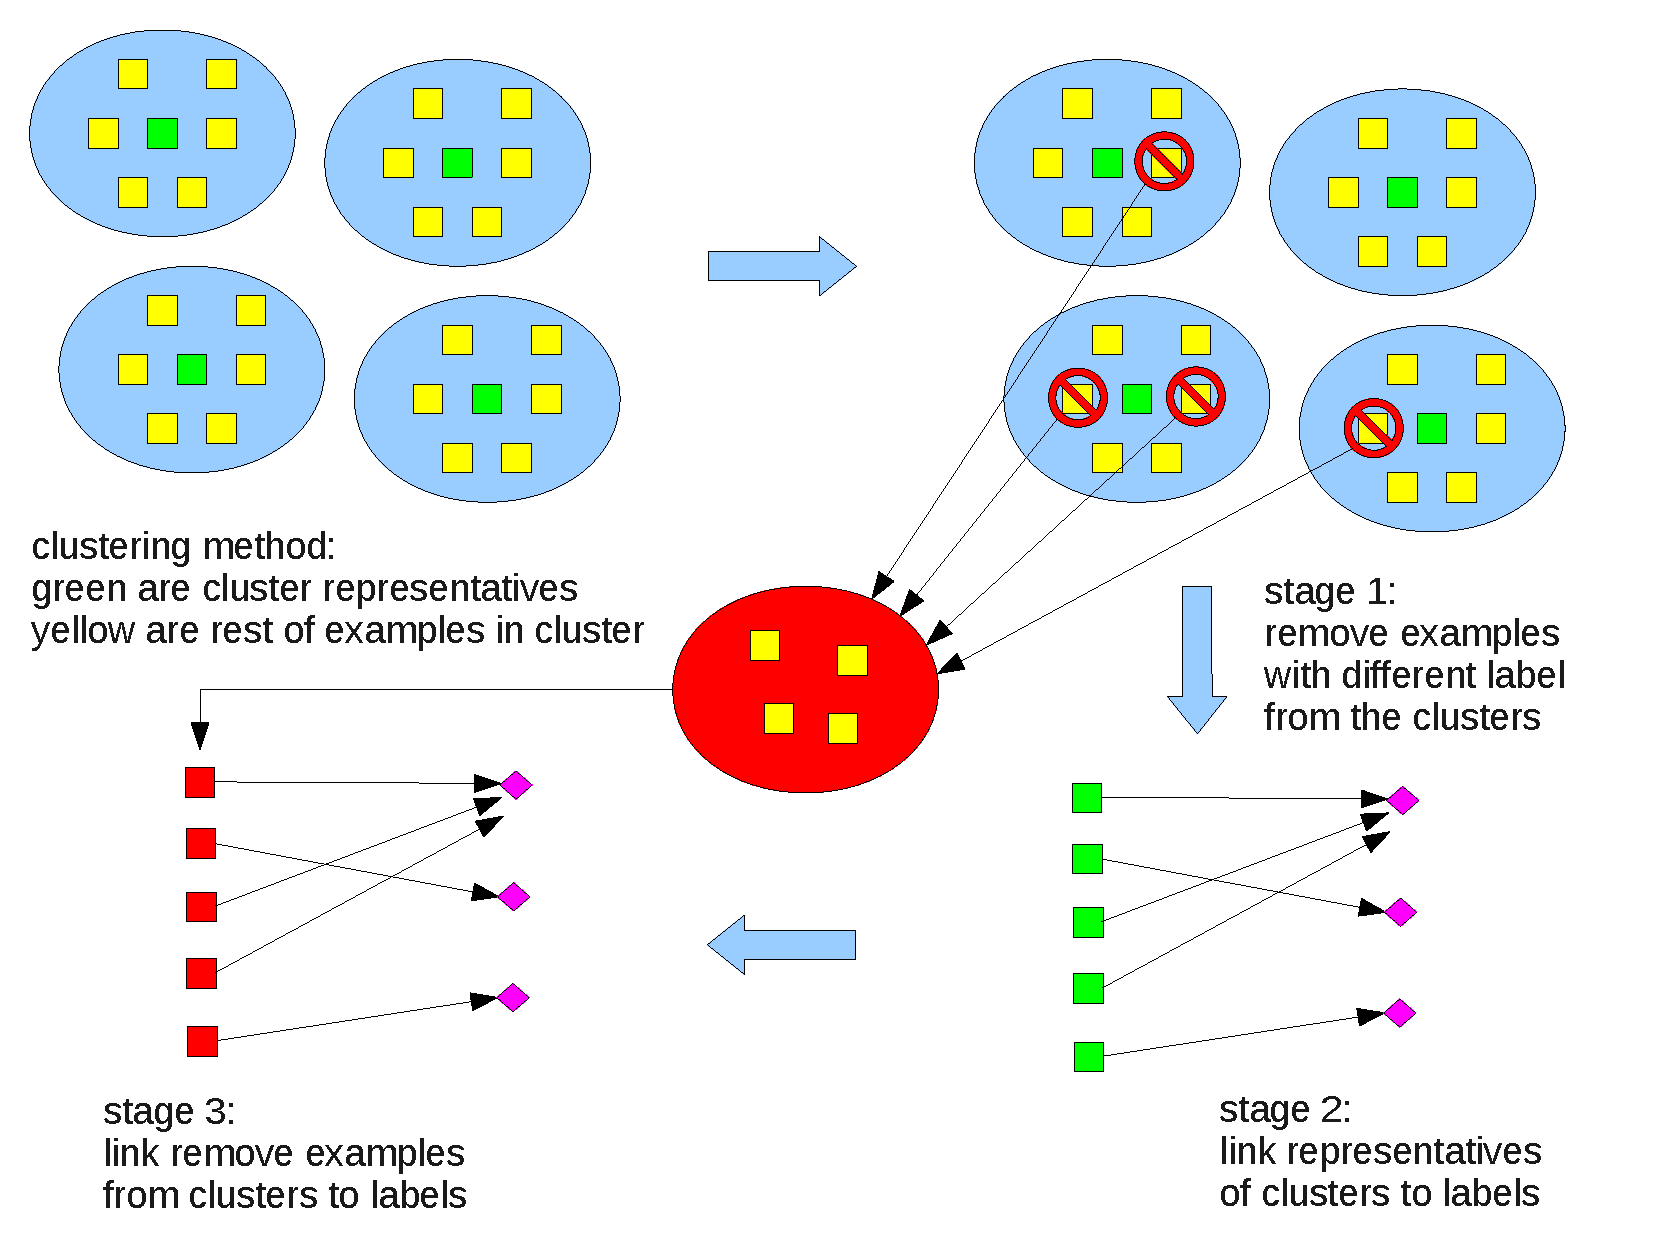
\includegraphics[width=3in]{schematicfigureclusteringmethod}
\caption{A schematic representation of the method we use to the annotate images with the support of a clustering method}
\label{fig:scheme}
\end{center}
\end{figure}

\subsection{Manual Groundtruth Annotation using Automatic Clustering}
%Manual annotation of images for the task of recognition can be time consuming work. 
In our project, we would like to obtain the names of different fish species that we observe 
in the underwater cameras. However, labelling thousands of images by hand is a time consuming process.
For clarity, in this paper we use the definition "cluster" for a group of images which are similar as determined by an 
automatic algorithm. The definition for "label" is a group of images which belong to the same category from 
the perspective of the human annotator and this group contains all the images in this category.
Hence we aim to improve this procedure by using a clustering method. 
Instead of giving a label for every fish, it is much faster and easier 
to check if a fish image is similar to another fish image. 
Note that the task of the annotator changes from typing in species name for each image to judging images clusters. 
Although the latter task can still be difficult, the images are processed in a batch mode and it
does not require as much domain knowledge as the former task.


In order to label an entire dataset of images using a clustering method, we have developed a strategy which
consists of three steps:
\begin{enumerate}
 \item  Cleaning the cluster, where we remove images which are not similar to the representative image
 \item  Merging the clusters, using the representative image of the cleaned clusters to link them to labels
 \item  Linking removed images from the cleaning stage to the labels. 
\end{enumerate}
 For fish, this means that a label includes all fish
of a certain species in the dataset.
\todo{Terms ``cluster'' and ``label'' alrady occured in the begining of the section. Are they refer to the 
same concepts? If so, it's better to explain them ealier; if not, it's better to change the names in previous text.}

In Figure~\ref{fig:scheme}, we show a schematic representation of the proposed method to annotate images. 
The blue oval describe the clusters, where the green images are the representative images in the cluster. Our
method consists of three stages, in the first stage we clean the clusters by removing the images that do not have
the same label as the representative image. In the second stage, we link the represenative images to a label
(shown as purple diamonds). In the third stage, we link the images which were removed from the cluster (shown as
red squares) to a label. However, whether one needs to perform the last stage depends if you want to label all 
the images in your dataset or if a large subset of all the images is sufficiet.
For comparison reasons we perform this stage, in order to make our method comparable with labeling every image
in the set individually. In the next sections, we will discussed the steps in more 
details together with the interface design. 
% 
\begin{figure}
\begin{center}
\includegraphics[width=3in]{selectdiffish}
\caption{This is the first interface for annotation that allows annotators to click on the images in the cluster that do not
below to the same label as the representative image on top of the page}
\label{fig:interface1}
\end{center}
\end{figure}
%

\subsection{Annotation interface for non-expert annotators}
For the first stage, we use the cleaning interface shown in Figure~\ref{fig:interface1}. In this case, the
representative cluster image is the image on top in the interface and the rest of the images in that cluster
are shown under this images. The annotator only has to select the images which are not correct and continue to
the next window. In our interface, we assume that people can deal with around 30 gallery 
images in a screen at one time (more images often requires extra work such as scrolling down).
Therefore our clustering method tries to obtain cluster of around 30 images. 
After cleaning all the clusters, there are basically three kinds of images in
the dataset: the representative cluster images, the images that belong to a cluster and the images that are not
part of a cluster.\\ 

\begin{figure}
\begin{center}
\includegraphics[width=3in]{selectfish}
\caption{This is the second interface for annotation that allows annotators to link a image to a label by clicking
on one of the gallery image which belongs to the same label as the image on top of the page or add a new label
by pressing the green plus button}
\label{fig:interface2}
\end{center}
\end{figure}
  
In the second stage, we are going to link the clusters to labels using the representative image . 
Notice that by linking these images, we also immediately link the images that belong to the underlying clusters. 
In many cases, some initial examples of labels are already in the database, which can be used in the interface shown in 
Figure~\ref{fig:interface2}. 
%
In this case, we simply pick the first representative image as a label. 
The annotator will then use the linking interface shown in Figure~\ref{fig:interface2} to link the next representative
image to this first label image.
However, it is also possible that there are no initial examples. In this case,
the annotator will create another label by pressing the green plus button. 
%
In the first case, the clusters are under the same label and linked. 
%
In the second case, a new label and representative label image are created. 
%In the previous step, we already mentioned that we let annotators deal 
%with around 30 gallery images, however if there are more than 30 labels, it becomes hard to show everything. 
%In our case, we are able to compute the similarity between images, allowing us to compute the most likely label
%given the image on top an ordering the images according to likeliness.
As mentioned in the previous step, ideally we would show 30 images per screen, so that 
the annotators do not have to perform additional actions such as scrolling down.
Similarly, in this step, when there exist more than 30 labels, it becomes hard to show everything
in one screen. Here, we rank the labels in the descending order
of their similarity to the top image. 

In the third step, we link the set of images that are not part of a cluster \todo{to a label?}. 
In this case, we use the same 
interface as in the previous step to link also these images to a label. 
Note that it is possible that there
are images in this set that do not belong to any label yet. 
(A speed-up can be achieved for large dataset if we recluster the images
and use both the first and second interface, however from a user-perspective switching these different 
interfaces can be confusing so in this work we only use the second interface to link them to clusters.)


\subsection{Annotation interface for expert annotators}
Since the final goal of the annotation is to assign a species name to each of the fish images, 
beside non-expert annotators' annotation over the fish clusters, we also need expert annotators
to assign species names to each of the clusters. 
%
As said before, experts are expensive and rare resources. Hence we use expert annotators to annotate
only a subset of our data.
The images annotated by the experts can be used as a validation set for the non-expert annotation.

The interface for expert annotators is similar to the first stage interface for the non-expert
annotators. See Figure~\ref{fig:expert}. Using this interface, the expert annotator first enters the species
name that applies to the majority of the images in a cluster in the top-right text box.
Once the name is entered, all images within the cluster are automatically assigned with the same species name. 
Then, the annotator is asked to select those images that do not belong to the cluster. 
By selecting these images, he/she can input the correct species names for them in the text box
under each image. In this manner, in the worst case, the annotator will have to manually assign a species
name to each of the images, i.e., when the clustering is so bad that each image within a cluster
contains a different fish species. In the best case, i.e., when the cluster is pure, 
the annotator only needs to enter the species name once.

After finishing annotation, we also include a questionnaire for the expert in order to collect
information such as which features the expert used to identify certain species. This type of information
may be a useful hint for selecting useful features when developing automatic methods for fish recognition.    

\begin{figure}
\begin{center}
\includegraphics[width=.5\textwidth]{expertlabel}
\caption{The interface for expert annotators. The expert enters the species name for the majority
of the images within a cluster, then select images that should not belong to this cluster and
input the correct species names for these images.}
\label{fig:expert}
\end{center}
\end{figure}

In our experiment, we invited 3 marine biologists, who have over 10 years research experience in the area
where the underwater video cameras are located. In order to obtain relatively high quality clusters, 
we manually constructed clusters over a small sub set of our dataset: 27 clusters over 524 images.
Since the sizes of clusters are very imbalanced,
for each cluster, we randomly sampled 30 images to be shown to the
biologists. In total 190 images 
were annotated by the biologists. 


For 82.6\% of the images, at least two biologists agreed on a species name;
for 56.3\% of the images, all biologists agreed on a name (including the
cases where two biologists agreed on a species name while
the third biologist indicated that he/she cannot identify the fish).
Further, if we look at the biolgoists' annotation per cluster, we see that
for different clusters, or in other word, different potential species of fish, 
biologists have different levels of agreement on their species names. 
From Figure~\ref{fig:expertdis} we see that for 9 out of 27 clusters
the biologists cannot agree on a species name for all images. A closer check-up
on the annotations shows that for 7 out of the 9 clusters, although the biologists
do not agree on the species names, they do agree on their family or genus names.
This suggests that for some fish images, it may be too difficult to recognize the 
species of the fish, while a family or genus level recognition may be more practical. 

\begin{figure}
\begin{center}
\includegraphics[width=.7\textwidth, height = 0.3\textwidth]{exp_disagree}
\caption{In each cluster, the percentage of the images where biologists disagree on their species names.
Here ``disagree'' refers to the situation where each biologist assigns a different name to the image, 
or all the biologists indicate that they cannot identify the species. 
%Clusters are ordered by their degree of experts' disagreement.
}
\label{fig:expertdis}
\end{center}
\end{figure}

\begin{figure}
\begin{center}
\includegraphics[width=.7\textwidth, height = 0.3\textwidth]{nonexp_error_nonstrict}
\caption{
In each cluster, the percentage of the images that at least 2 biologists suggest that
these images should be removed from the cluster.
%Clusters are ordered by their degree of experts' disagreement.
}
\label{fig:nonexp_error}
\end{center}
\end{figure}
  
Futher, we compare the manual clustering results to the biologists' annotation in order
to check the performance of non-expert in grouping fishes into species based on their visual
similarity. In Figure~\ref{fig:nonexp_error} we show the percentage of ``errors'' the non-experts
made according to biologists' judgement, where an ``error'' refers to the case when at least 
two biologists indicate that a image should be removed from a cluster. We see that in most
of the cases, 21 out of 27 clusters, the groups of fishes created by the non-experts are 
approved by the biologists, which suggests that it is promising to use non-experts to identify
fish species (without actually knowning the names of the species) based on visual similarity.
Another observation we have here is that, if we compare Figure~\ref{fig:nonexp_error} to 
Figure~\ref{fig:expertdis}, we see that in many cases, while the non-experts have low error rate
in identify a cluster, the biologist have difficulty to agree on a species name for the cluster. 
For instance, in the case of cluster 3, 4, 5, 6, etc,.
This observation suggests that although it is promising to cluster fish images into visually similar
groups, it is not necessarily easy to associate this cluster to a specific label, in particular at
the species level.   


\todo{@Bas: why in my judgements 190 imgages are labeled by the biologists, but you only have 159? 
Did you do some sort of filtering? If we count the images that have at least two biologists agree on
a name, then it's 157.}



\todo{In case you are confused when checking the database: in the database the cluster version 1 has
28 clusters, however, cluster 16 is empty. In the paper, I removed the empty cluster, so from cluster 17 on, 
all the cluster id corresponds to the cluster id-1 in the database}

\subsection{Obtained annotations}
\todo{I think we need to at least briefly discuss how many images we annotated, how much time 
it takes, how we arrange people to do this (e.g., at least 3 non-expert to annotate), 
disagreements, evaluation results on the experts' subset, etc.}

At the moment, we have a first dataset of 3678 fish images, where 159 fish image have been given
a species name by the marine biologists. We found 6 users willing to annotate the entire database
of fishes for us using the clustering method to support them in their efforts. Based on the 
labeling of the biologists, we found out that the average user performance is 87.6\% correctly
labelled fish. There is however a large difference between people who saw the fish images
for the first time and people who are part of this project having observed some of the fish before.
The lowest user performance is 68.8\%, where this person basically annotated different species
that look similar to the same category. For users, it is often very difficult to determine if
fish belong to a different species or not, because appearances of the fish like the colour can
change due to illumination conditions. Another difference between users is their decision to 
ignore the fish image because you can not clearly identify fish basd on the images or the images
contains multiple fish. Some users used this ignore options very frequently, while other users
used it rarely. 

\begin{figure}
\begin{center}
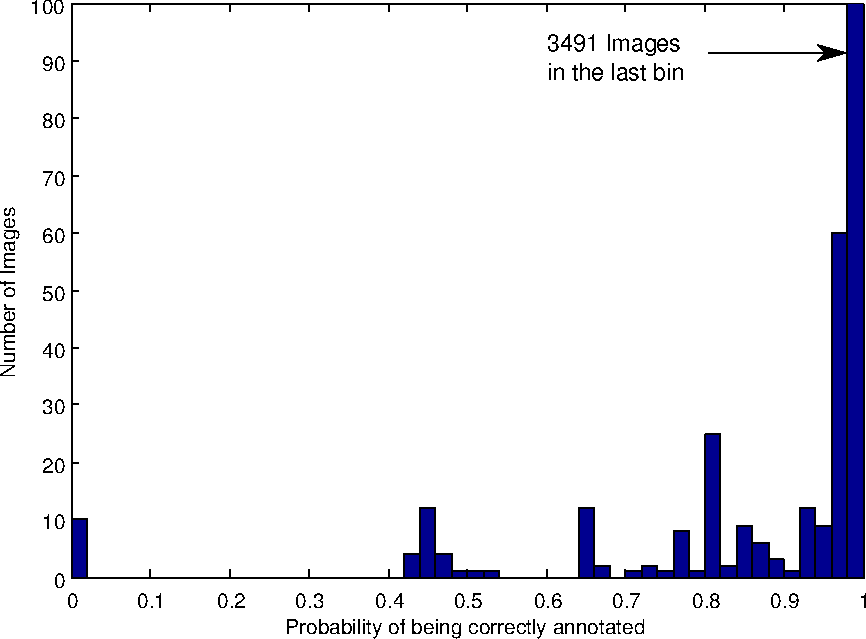
\includegraphics[width=3in]{distributionofdataset2}
\caption{We show the distribution on the probabilities that a images labelled by all users
is correctly, there are in this database however still a lot of disagreements between user. 
This images can be communicate to the marine biologists, for now we exclude them from the
dataset for training model and evaluation of our methods.}
\label{fig:distributionofdata}
\end{center}
\end{figure}

We combined the different labels given by all the users using the probabilities that the user
correcty labelled the fish measured using the biologists annotations. If user agreed on the label
the probabilities become very high while with disagreements results become much lower. In
Figure \ref{fig:distributionofdata}, we show the distributions on the user's disagreements,
in most cases however user do agree which can be observer in the last bar. In more than
90\% of the images, the probability of being correctly labelled is greater than 99.9\%.\\ 

We also look at the profit that we obtained by labelling using a clustering methods. Let us assume
that a user labels everything correctly. For the first interface, we need $\frac{M}{30}$ screens,
assuming $M$ is the number of image and that we show around the 30 images. For the second 
interface, we need screens to link all the clusters, where $C$ is the number of clusters and we need
to label all the images that do not have the same label as the representative images, let us
denote this by the number $R$, where for our clustering methods this was around $R = 300$. 
In order to measure the time it takes a user to label,
we asked one user to label images non-stop for us, where the average time in which he 
took annotating a screen in stage 1 is $T_{1}=19.7$ seconds and for stage 2 this was 
$T_{1}=7.3$ seconds. Given the Equation~\ref{eq:time} below we can easily estimate how much time 
it will take users, notice that labelling the entire dataset using the second interface 
will take $MT_{2}$. 

\begin{equation}
 \textit{time} = \frac{1}{30}MT_{1} + CT_{2} + RT_{2} \label{eq:time} \\
\end{equation}
\begin{equation}
 \textit{clicks} = \frac{1}{30}M + 2C + 3R \label{eq:clicks} \\
\end{equation} 

Equation~\ref{eq:clicks} estimates the number of click necessary to label the entire database,
In the first interface user need to click on very incorrect image $R$ and to go the next
screen users also need to click. We have add this to the number of mouse clicks required
for the second interface which is two mouse clicks, one to select the images and one to 
go to the next screen. If we have to annotate all screen using the second interface we
end up with $2M$ clicks, based on these equations it can be shown that with a good
performing clustering method (determining by the value $R$) large gains in time and number
of clicks can be obtained for annotating a dataset. \\

\begin{comment}
\subsection{Clustering Method}\label{sec:clustermethod}

The fish clustering method start from the assumption that the detection and segmentation of the 
fish is correctly performed. This is not neccessary, however, in previous section we already obtained
groundtruth data for detection and segmentation, which we use for the fish clustering methods. In the
case that we do not have groundtruth data we can use visual inspection to remove failures in the 
segmentation from the dataset, this is however more time consuming.\\
In order to cluster fish, we need a method which allows us to discover new species in the dataset.
The clustering method also needs to be invariant against a lot of variantions because of the 
uncontrolled nature of the video recording. The last property of the clustering methods is that it
will be able to deal with objects which are quiet similar, as suppose to most methods in image 
retrieval with cluster classes with are quiet dissimilar (car, building, people, etc). Our 
clustering method is very similar to the method describe in \cite{goldberger_unsupervised_2006}, especially in the way that this method  
measures the similarity between images. In order to cluster the images, we use Affinity Propagation \cite{frey_clustering_2007} 
instead of \cite{goldberger_unsupervised_2006}, because this is faster and more scalable with larger databases.\\
In order to represent every image, we fit a Guassian Mixture Model (GMM) to each of the seperate fish feature. The
GMM are fitted using the Expectation Maximalization algorithm described in \cite{zivkovic_recursive_2004}, which uses 
Minimum Description Lenght to automatically determine the number of Guassian density functions. We use
GMM because they allow to compare unseen fish feature. 
In new cases, a new feature (like a certain color) will be described using its own Guassian density functions. In order
to model fish, the most important features of fish are the color, texture (spot,strips,etc) and shape.
In the case of color, we transform all the pixel value of the segmented fish to HSV (Hue, Saturtion, 
Value), for the Hue channel two values are used, namely the sine and cosine of the Hue channel. This removes the big 
difference between the different red values because of the cylindrical color definition. From these 
4 dimensional data points, we then obtain a GMM using \cite{zivkovic_recursive_2004}. For the texture, a GMM is fitted to the magnitude
and the orientation of the Canny filter at each pixel in the segmented fish. We also fitted a GMM on the curvature
scale space representation of the fish contour, where we use the points on lines given by the curvature 
scale space of the fish contour input data points. The advantage of using the curvature scale space is that
it gives an invariant representation for most affine image transformations on the contour.\\
In \cite{goldberger_unsupervised_2006}, the similarity between two GMM is determined by using a Monte-Carol
simulation to approximate the Kullback-Liebler divergence:

\begin{equation}
 D(f \Vert g) = \int f \log \frac{f}{g} \approx \frac{1}{N} \sum_{t=1}^{N} \log \frac{f(x_t)}{g(x_t)} 
\end{equation}
\begin{equation} 
 S(f,g) = D(f \Vert g) + D(g \Vert f)
\end{equation}


We use the symmetric version of the KL-divergence (Equation 2) to measure the similarity between different 
fish images. Given the three different kind of features, we obtain three different KL-divergence which
we sum together to get the final similarity measure. Instead of using the clustering approach proposed in \cite{goldberger_unsupervised_2006}, 
we use Affinity Propagation \cite{frey_clustering_2007} which scales better on large image databases. This is a graph 
based clustering method, which can automatically find clusters given a matrix of similarity measurements. This clustering method passes
messages around to determine the responsibility and availability. The message of responsibility between point
$i$ and $k$ reflects how well suited point $k$ to represent point $i$. The availability message between point
$i$ and $k$ indicates how appropriate it is for point $i$ to choose point $k$ as representative. The final 
outcome of the clustering method is are clusters of fish images which have one images as a representative 
image. The representative image is important in our interface because we use this image to link the clusters together.
Although the clustering method should not matter, speed up in the manual annotation can be achieved if the 
clusters and the similarity between fish are of better quality. Because \cite{frey_clustering_2007} gives us representative image
for each cluster, this does not mean that other clustering methods can not be used. For instance by using K-means
clustering, it is easy to select the images closes to the mean as representative, but as using a random
images in the cluster as representative should also work. 
 
\subsection{Manual Annotation using Automatic Clustering}

Manual annotation of image for the task of recognition can be time consuming work. In our project, we would like to
obtain the different species which we observe in the underwater cameras. However, labelling thousands of
images by hand is a time consuming operation, so we improve this task by using a clustering method. Instead 
of giving a label for every fish, we agrue that it is much faster to check if a fish image is similar to another
fish image. Notice that the task of the user change from typing fish names to judging images. Although this task 
can still be difficult, it does not require as much domain knowledge as the previous task.\\
In order to label an entire dataset of image using a clustering method, we have developed a strategy which
consists of three steps:
\begin{itemize}
 \item Cleaning the cluster, where we remove images which are not similar to the represenative image
 \item Merging the clusters, using the representative image of the cleaned clusters to link them to labels
 \item Linking removed images from the cleaning stage to the labels. 
\end{itemize}
In this paper, we use the definition cluster for a group of images which are similar determine by a 
automatic algorithm. The definition for label is a group of images which are similar to the human annotator
and this group contains all the similar image in the entire set. For fish, this means that in a label we obtain all fish
of a certain species in the set. \\

\begin{figure}
\begin{center}
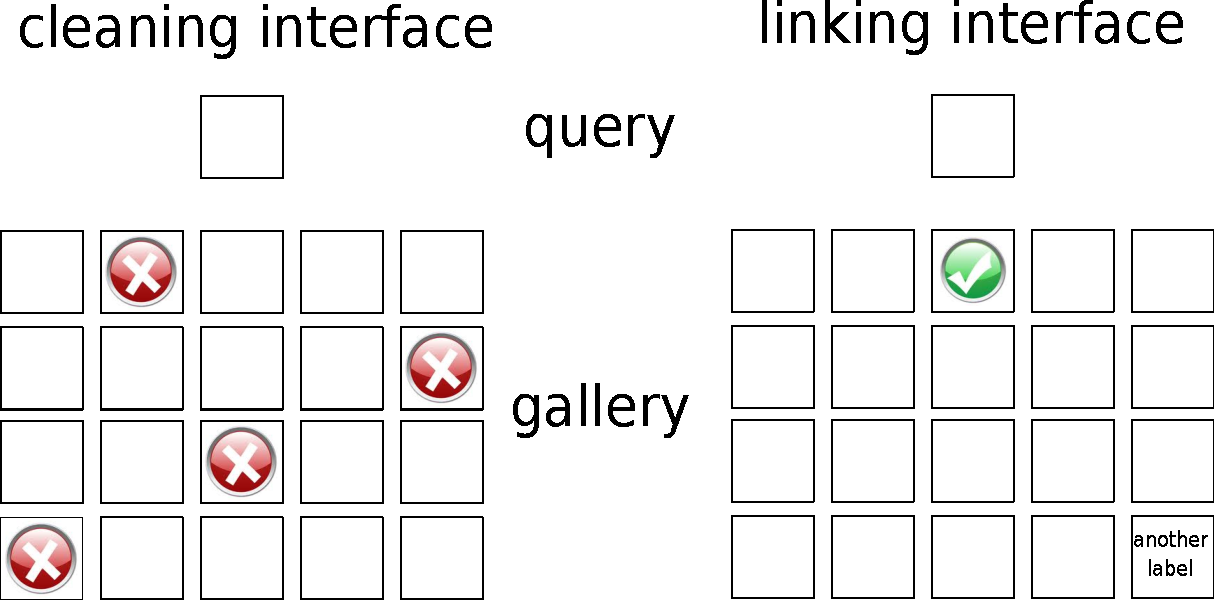
\includegraphics[height=3in]{images/interfacesresizedv2}
\caption{This are the two interface which we use to annotated the images, the first interface allows us to clean the clusters by
clicking on gallery images that do not below to the same label as the query image, the second interface is to link the clusters
together allowing a person to click one gallery image with the same label. In the second interface, we assume that there are no
images with the same label in the gallery and that it is possible to indicate that there is no image with the same label in the
gallery using the Another Label button (right-bottom)}
\label{fig:interfaces}
\end{center}
\end{figure}

For the first step, we use the cleaning interface shown in Figure~\ref{fig:interfaces}. In this case, the
representative cluster image is the query image in the interface and the rest of the images in that cluster
are put in the gallery. The user only has to select the images which are not correct and can continue to
the next window after finishing this task. In our interface, we assume that people can deal with around the 30 gallery 
images in a screen at once (more images usually requires actions like scrolling down which is also extra work). So
our clustering method trieds to obtain cluster of around the 30 images and people can select the images which
are not part of the clusters. After cleaning all the clusters, there are basically three kind of images in
the dataset. The representative cluster images, the images that belong to cluster and the images that are not
part of a cluster.\\   
In the second step, we are going to link the clusters using the representative cluster images to labels. Notice
that by linking the clusters, we also immediately link the images that belongs to that cluster. In order to link
the representative cluster images, we are going to link all the representative cluster images to representative 
label images. In many cases, some initial examples of labels are already in the database which can be used to 
link to the representative cluster images. However, it is also possible that there are no initial examples. In 
this case, you can just pick the first representative cluster image as first representative label image. The user
will then use the linking interface shown in Figure~\ref{fig:interfaces} to link the next representative cluster
image to either first representative label image or to another label. In the first case, the clusters are under
the same label and will be linked. In the second case, a new label and representative label image are created. In the previous step,
we already mentioned that we let users deal with around the 30 gallery images, however if there are more than 
30 labels, it becomes hard to show everything. In our case, we are able to compute the similarity between images,
allowing us to compute which representative label image are most likely to be the representative cluster image.\\
In the thrid step, we link the set of images that are not part of a cluster. In this case, we use the same 
interface as in the previous step to link also these images to a label. Notice, that it is possible that there
are images in this set that do not belong to any label yet. (A speedup can be achieve in this step if we use
a combination of the first and second interface. There are probably a lot of images that match almost equally well
to two label and are just in the first stage cluster with the wrong label. Using the first interface to link them 
to the second most probable label can achieve a speed up, however from a user perspective switching these different 
interfaces can be confusing so in our initial test we only use the second interface to link them to clusters.)

\subsection{Simulation Program}

We create a simulation program to see how much windows and clicks one needs to label a set of $3678$ fish images, from which
we already obtain the labelling. In a lot of labelling programs, we label each image individually so we need to view
$3678$ windows, type in the correct name or select the name from a dropdown box. We usual need to confirm our finding
with a click which takes us to the next window. If we improve this interface slightly for our problem, we can
use basically the linking interface in Figure~\ref{fig:interfaces} to label each image seperately. This will take $3678$ windows but only 
$3678\times2$ mouse clicks assuming that you have to click on the correct gallery image and a confirm button to
go to a next window. Here, we did not take into account that you have more than $30$ labels you need more screens anyway.\\ 
In our new program, we want to minimize the number of screens and clicks. For the cleaning interface, this means 
that the users normally click all incorrect image and gives a final click to conform and go to a next screen. For
the linking interface, we already explained the procedure needs only 2 clicks for each window. In the case, that
we combine our new proposed interface with random selection of cluster and similarity score between images, we need a total of 6535 clicks and 1358 screens 
to annotate the entire database. In the case, that we use the clustering method describe in Section~\label{sec:clustermethod}, 
we only need 1558 clicks and 621 screens. This is a large improvement of the previous proposed interface and the method 
without using clustering. Since a lot of the crowdsource website let you pay for the number of clicks a user have 
to perform these kind of strategies might be an interesting tools to get good results in a cheaper way.\\

\subsection{Possible Todo List}

\begin{itemize}
 \item combining labeling ... very easy with simulation program at the moment
 \item majority voting ... disagreement solutions .... can use simulation programs
 \item different kind of users mistake .... random and systematic 
 \item how to use experts? for instance to check final labels or solving user disagreements or testing user accuracy
 \item creating a real interface for labelling (Jiyin on holiday, until end this month)
 \item different database .... (flower database)
 \item bayesian network to describe label certain (or other model to describe certainty and quality of normal label and labeling with our new approach)
 \item write paper for Concetto and CVPR
\end{itemize}

majority voting ... disagreement solutions .... can use simulation program
keeping expert in the 

\end{comment}

% \subsection{Some first work on Jiyin in estimation number of screen and clicks}
% 
% \todo{I have a feeling that the simulation part can be modeled analytically. e.g., the number of clicks is a function
% of the number of clusters, number of singletons, given that users don't make mistakes and want to go back.}     
% 
% \todo{[Here is my initial thoughts about modeling the effort of users of my interface]}   
% 
% The interface consists of two separate screens, let us call them $S1$ and $S2$.
% $S1$ is used for merging clusters. It lists all the $N$ clusters generated by the clustering algorithm.
% Each cluster has a cluster number and a dropdown manu next to it. For each cluster a user can 
% choose a cluster number from the dropdown manu and merge current cluster with the selected one. 
% The interface then contains $N-1$ clusters. In other words, every merge happens between two clusters.
% %
% $S2$ is used for processing singletons (images that are marked at ``not in cluster'') during the cleaning
% stage. It contains two parts. In the top part, we show all the clusters identified by the clustering 
% algorithm except the one where the singleton was assigned to, i.e., in total $N-1$ clusters are included. 
% On the bottom part, we show one singleton image and two buttons ``new cluster'' and ``next''.
% The user compares the image and the pre-identified
% clusters and decide if the image belong to one of the clusters by clicking that cluster, or decide that it
% does not belong to any of the clusters by clicking ``new cluster''. 
% Then by clicking ``next'' the user proceeed to judge next singleton. If the current image creates a ``new
% cluster'', in the next screen, the top part will contain $(N-1)+1$ cluster, including the newly created one.
% %
% When showing a cluster, we show randomly sampled 3 images from that cluster.  
% 
% Let $N$ be the number of clusters generated by the clustering algorithm, $M$ be the number of singletons, 
% we evaluate the effort of a user spend on judging a set of images using the following three criteria:
% number of screens shown to the user $E_s$, the number of clicks needed $E_c$ and the number of comparisons
% between the clusters or between a singleton and the clusters $E_v$.     
% 
% The number of screens needed is rather simple to be determined: $S1$ shows once and $S2$ shows for each of
% the singleton, therefore:
% \begin{equation}
%  E_s = 1 + M
% \end{equation}
% 
% The number of clicks depends on the following factors: the number of identified clusters $N$, the number
% of singletons $M$, and the number of clusters $K$ perceived by the user. Assume the users have an overview
% of all the clusters on $S1$ and make up their mind before clicking the dropdown manu to merge clusters. 
% That is, they do not change their mind and un-merge the merged clusters. The number of clicks needed
% can be determined as follows.
% \begin{equation}
%  E_c = N-K + 2M-1
% \end{equation}
% where $N-K$ is the number of clicks needed in order to merge $N$ clusters into $K$ clusters, and 
% $2*M-1$ is the number of clicks needed to process the $M$ singletons. On each screen, the users
% need to click either an existing cluster or the button ``new cluster'', then they need to click 
% the ``next'' button except for the last singleton image. Further, $1\le K \le N$. In the best 
% case where $K=N$, no clicks are needed on screen $S1$ and therefore $E_c=2M-1$. 
% In the worst case where $K=1$, the total clicks needed are $E_c = N + 2M - 2$.
%   
% The number of comparisons a user need to complete the task can be estimated as follows.
% 
% On screens $S2$, assume that a user would stop comparison after he find a first match at cluster $n$, 
% we have the following situations. In the worst case, each singleton forms a new cluster, and on each
% screen the user needs to compare each of the existing cluster to the singleton and therefore
% $E_v(S2) = \sum_{i=0}^{M-1} (N-1+i)$. In the best case, each singleton belongs to the first cluster the user
% compares and the number of comparison needed is $E_v(S2) = M$. 
% As the worst and best situation are unlikely to happen, it is more interesting to consider the average situation.
% 
% \begin{equation}
%  E_v(S2) = \sum_{i=1}^M 
% \end{equation}
% 






     


 
